\documentclass[11pt, a4paper]{article}

\usepackage{geometry} 
\usepackage{epsfig}
\usepackage{epstopdf}
\DeclareGraphicsRule{.tif}{png}{.png}{`convert #1 `dirname #1`/`basename #1 .tif`.png}
\setlength{\oddsidemargin}{0cm}
\setlength{\evensidemargin}{0cm}
\setlength{\topmargin}{-1cm}
\setlength{\textheight}{23cm}
\setlength{\textwidth}{16cm}

\pagestyle{headings}

\newcommand{\BAT}{{\sc BAT}}
\newcommand{\versionno}{0.2}
\newcommand{\version}{version~\versionno}
\newcommand{\Version}{Version~\versionno}

%--------------------------------------------------------

\begin{document}

% --------------------------------------------------------
% title
% --------------------------------------------------------

\thispagestyle{empty} 

\begin{figure}

\leftline{
\includegraphics[scale=0.25]{bat.eps} 
\hspace{9.0cm} 
\Version}

\end{figure}

\title{\BAT\ - A {\sc Bayesian Analysis Toolkit}}

\author{A.~Caldwell$^{1}$, D.~Kollar${^2}$, K.~Kr{\"o}ninger$^{3}$}

\maketitle

\begin{center}
$^{1}$~Max-Planck-Institut f{\"u}r Physik, Munich \\ 
$^{2}$~CERN, Geneva
$^{3}$~II.~Physikalisches Institut, Universit{\"a}t G{\"o}ttingen \\ 
\end{center}

\thispagestyle{empty} 

\begin{abstract} 
The Bayesian Analysis Toolkit, \BAT, is a software package designed to
help solve statistical problems encountered in Bayesian
statistics. Allowing to formulate models and their parameters, the
main purpose of the toolkit is to provide methods to solve the
numerical optimization and integration. It features the possiblity to
estimate parameters and to compare models. A procedure to estimate the
goodness-of-fit is included and based on ensemble tests. 
\end{abstract} 

\pagebreak 

% --------------------------------------------------------
% table of contents 
% --------------------------------------------------------

\thispagestyle{empty} 

\tableofcontents

\pagebreak 

% --------------------------------------------------------
% introduction
% --------------------------------------------------------

\section{Introduction}

The goal of data analysis is to compare model predictions with data,
and draw conclusions on the validity of the model as a representation
of the data, or to estimate best-fit parameter values within the
context of a model. The paradigm for our data analysis package is
shown in Fig.~\ref{fig:scheme}.  Here, the model M can range from a
model purporting to represent nature (e.g., the Standard Model in
particle physics) to a simple parametrization of data useful for
making predictions or for summarizing data.  In the latter case, the
intermediate steps in the figure would be skipped. \\ 

\begin{figure}[htbp] %  figure placement: here, top, bottom, or page
\centering
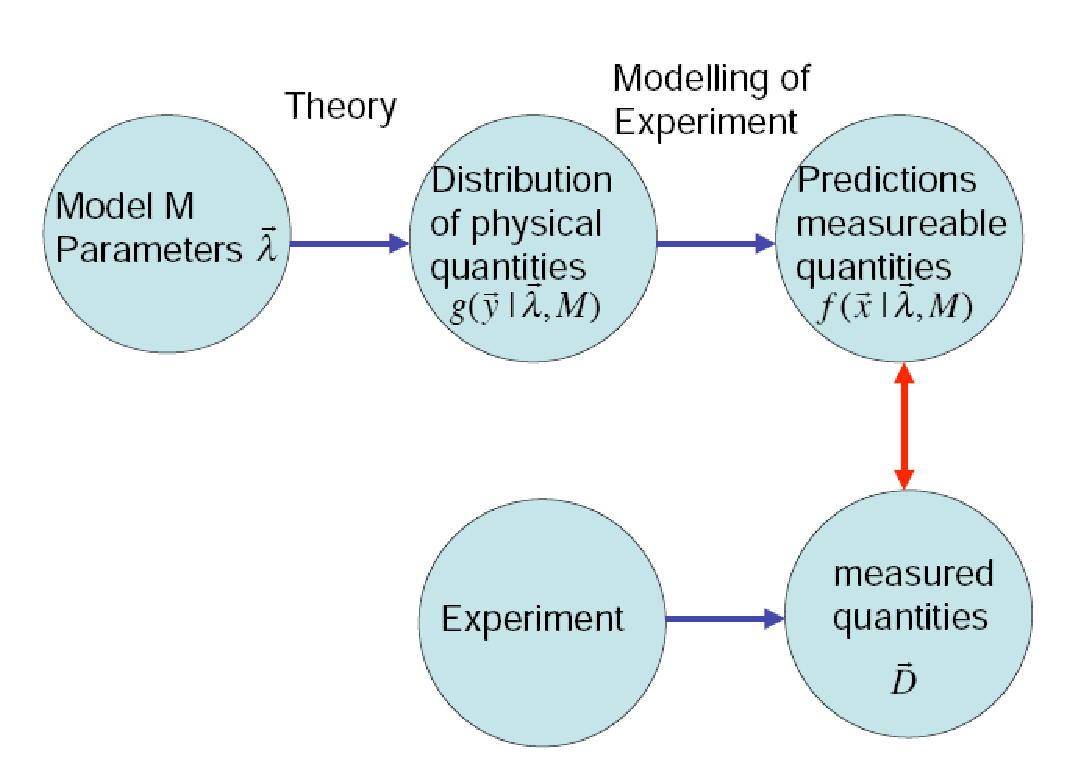
\includegraphics[width=0.75\textwidth]{scheme.eps} 
\caption{Paradigm for data analysis.  Knowledge is gained from a
comparison of model predictio ns with data.  Intermediate steps may be
necessary, e.g., to model experimental conditions.}
\label{fig:scheme}
\end{figure}

Note that the model provides `Direct Probabilities'; i.e., frequency
distributions of possible outcomes of the results were one to
reproduce the experiment many times under identical conditions.  The
function
%
\begin{equation}
f(\vec{x}|\vec{\lambda},M)
\end{equation}
%
gives the probability (density) of getting result $\vec{x}$ assuming
the model $M$ and parameters $\vec{\lambda}$\footnote{The modelling of
the experiment will usually add extra parameters and assumptions,
which then also appear as arguments}.

The probability of a model, $M$, will be quantified as $P(M)$, with:
%
\begin{equation}
\label{eq:norm}
0 \leq P(M) \leq 1
\end{equation}
%
while the probability (density) of the parameters are typically
continuous functions.  The probability (densities) satisfy
%
\begin{eqnarray*}
P(\vec{\lambda}) & \ge & 0 \\
\int P(\vec{\lambda}) d\vec{\lambda} &=&1 \;\; .\\
\end{eqnarray*}

In the Bayesian approach, the quantities $P(M), P(\vec{\lambda})$ are
treated on the same footing as the direct probabilities, although they
are not in any sense frequency distributions and must be determined
via inductive reasoning.  The procedure for learning from experiment
is:
%
\begin{equation}
P_{i+1}(\vec{\lambda},M) \propto f(\vec{x}=\vec{D}|\vec{\lambda},M) P_{i}(\vec{\lambda},M) 
\end{equation}
%
where the index represents a `state-of-knowledge'.  

In order to satisfy Eq.~\ref{eq:norm}, we set
%
\begin{equation}
P_{i+1}(\vec{\lambda},M) =\frac{f(\vec{x}=\vec{D}|\vec{\lambda},M) P_{i}(\vec{\lambda},M)}
{\sum_M \int f(\vec{x}=\vec{D}|\vec{\lambda},M) P_{i}(\vec{\lambda},M) d{\vec{\lambda}}}
\end{equation}
%
We usually just write $P_i=P_0$, and this quantity is called the
`prior'.  The function $f$ does not need to be normalized, since the
overall normalization is taken care of automatically.  When $f$ is
viewed as a function of $\vec{\lambda}$ for fixed $\vec{x}=\vec{D}$,
it is known as the likelihood.

\subsection{Validity of Model}
\label{subsection:validity}

The following quantity is proposed to evaluate the validity of a
model,$M$, (including any modelling of the experimental conditions):
%
\begin{equation}
p=\int_{f(\vec{x}|\vec{\lambda^*},M)<f(\vec{x}=\vec{D}|\vec{\lambda^*},M)} \frac{f(\vec{x}|\vec{\lambda^*},M) d\vec{x}}{\int f(\vec{x}|\vec{\lambda^*},M) d\vec{x}}
\end{equation}
%
where $\vec{\lambda^*}$ are the optimal values of $\lambda$ (e.g.,
best-fit values). The quantity $p$ is just the `tail-area' probability
to have found any result with smaller $f$ than that given by the
measured data, given $M,\vec{\lambda^*}$.  This quantity is analogous
to the usual $\chi^2$ probability, but is more general since it can be
used for any function $f$.

\subsection{Parameter estimation}
%
Parameter estimation is performed while keeping the model fixed.  In
this case, we write
%
\begin{equation}
P_{1}(\vec{\lambda}|M) =\frac{f(\vec{x}=\vec{D}|\vec{\lambda},M) P_{0}(\vec{\lambda}|M)}
{\int f(\vec{x}=\vec{D}|\vec{\lambda},M) P_{0}(\vec{\lambda}|M) d\vec{\lambda}} \;\; .
\label{eqn:BayesTheorem}
\end{equation}
%
The output of the evaluation is a (multidimensional) normalized
probability density for the parameters, including all correlations.
This output can be used to give best-fit values, probability intervals
for the parameters, etc.

The scheme for updating knowledge, as written down here, is quite
general and straightforward.  There can be difficulties in
implementation when dealing with multi-dimensional spaces, and the
toolkit presented here is designed to help the user solve these
technical issues.  As a general statement, it should be obvious that
the `garbage in, garbage out' rule applies.  It is up to the user to
carefully define the model, parameters, predictions, and priors.  The
BAT program will then be useful as a tool for model testing and
parameter estimation.

In the following, we will give several examples of parameter
estimation and model testing to make the ideas more concrete.

% --------------------------------------------------------

\subsection{Example uses of Bayesis Inference} 
\label{subsection:exampleuses} 

Describe in general terms how a problem is formulated. Some examples:

\paragraph{Structure functions} 

\paragraph{Neutrinoless double beta-decay} 

Neutrinoless double beta-decay ($0\nu\beta\beta$) is rare nuclear
process predicted to occur if the neutrino is a Majorana
particle~\cite{Yao:2006px}. It has two electrons and no neutrinos in
the final state. Experiments searching for $0\nu\beta\beta$-decay of
$^{76}$Ge measure the ionization energy deposited in Ge-semiconductor
detectors. Since the energy released in the decay, the $Q$-value, is
fully transferred to the electrons the experimental signature of such
a decay is a sharp line at that energy. In experiments like
GERDA~\cite{Schonert:2005zn} the background in the region of interest
is expected to be flat. \\ 

\noindent 
Due to the small number of signal events predicted special care has to
be taken when analyzing the measured energy spectrum. Common
approximations which are only valid for a laarge number of events
cannot hold in that case. A spectral analysis based on Bayes' Theorem
has been developed for that purpose~\cite{Caldwell:2006yj}. The
sensitivity of the GERDA experiment has been evaluated using Monte
Carlo techniques. A simplified version of the analysis is given as an
example in the code (see Section~\ref{section:example03}). 

\paragraph{Cosmological models} 

% --------------------------------------------------------

\subsection{Requirements} 

The BAT toolkit was written to assist the user solving statistical
problems in Bayesian inference. Of course the user has to be able to
formulate the problem encountered. This means that the user has to
provide a valid model together with all parameters and limits of the
parameters. It is obvious that BAT can only help solve the
mathematical part of the statistical analysis, in particular the
numerical integration and optimization.  \\

\noindent 
During the run-time of the program the user can adjust several
parameters for numerical integration and optimization. These
parameters influence the performance of calculation and are not
connected to the mathematical formulation of the problem
encountered. In Section~\ref{section:analysis}, the steps of the
analysis chain are discussed and the adjustable parameters
introduced. It should be noted that these parameters are model
dependent and need to be adjusted to each problem separately. 

% --------------------------------------------------------
% >>>>>>>>>>>>>>>>>>>>>>>>>>>>>>>>>>>>>>>>>>>>>>>>>>>>>>>>
% installation 
% >>>>>>>>>>>>>>>>>>>>>>>>>>>>>>>>>>>>>>>>>>>>>>>>>>>>>>>>
% --------------------------------------------------------

\pagebreak 

\section{Installation} 

\subsection{Platforms}

\BAT\ has been developed on Linux machines running different distributions
and different versions of the kernel and gcc. As far as we know there
is nothing distribution dependent inside of \BAT. However, we have not
yet started to systematically check for compatibility and
portability. This is planned for future releases of \BAT. For the
moment the only statement we can do here is that if you don't have a
too old or too specific installation of Linux you should be able to
compile and use \BAT\ without problems. \\ 

Windows is not supported for the moment. \\ 

\subsection{Dependencies}

\paragraph{ROOT:} 
ROOT is an object oriented data analysis framework. You can obtain it
from~\cite{ROOTweb}. To compile and run BAT you
will need a ROOT version 5.16 or later. Please, check your Linux
distribution for the availability of precompiled packages on your
system. Mostly used distributions nowdays have the ROOT packages
available

\subsection{Recommendations}

\paragraph{CUBA:}
CUBA~\cite{CUBA} is a library containing general purpose
multidimensional integration algorithms. It can be obtained
from~\cite{CUBAweb} . In this version BAT no longer depends on CUBA
and you can compile and run without it. However, the use of CUBA is
recommended as it provides integration routines tuned for performance,
which are very usefull for integration in problems with large number
of dimensions. \\ 

Note: Since version 1.5 the compilation of CUBA no longer crashes if
you don't have Mathematica installed. To compile and install CUBA
libraries use commands 'make lib ; make install'.

\subsection{Installation procedure}

Unpack the tarball containing the BAT source usually named like
BAT-x.x.tar.gz (here x.x is the version number) using command
%
\begin{verbatim}
tar -xzf BAT-x.x.tar.gz
\end{verbatim}
%
A directory called BAT-x.x will be created containing the source code.
Enter the directory and run the configuration using commands
%
\begin{verbatim}
cd -x.x
./configure
\end{verbatim}

This will check your system for all components needed to compile BAT
and set up the paths for installation. You can add option
\verb|--prefix=/path/to/install/bat| to \verb|./configure| to specify
the the prefix to the BAT installation path. The BAT library files
will be installed to \verb|$prefix/lib| and the include files to
\verb|$prefix/include|. Default installation prefix is
\verb|/usr/local|. \\ 

The configure script checks for ROOT availability in the system and
fails if ROOT is not installed. You can specify the ROOTSYS directory
using \verb|--rootsys=/path/to/rootsys|. \\ 

The configure will also search for \verb|libcuba.a| and \verb|cuba.h|
in the system.  The \verb|libcuba.a| has to be available in the
standard system library search path. You can specify the \verb|cuba.h|
location using \verb|--with-cuba-path=/path/to/cuba/header|.

After successful configuration run
%
\begin{verbatim}
make
make install
\end{verbatim}
%
to compile and install BAT. Note that depending on the setting of
installation prefix you might need root priviledges to be able to
install BAT. If you are installing BAT e.g. in your \verb|$HOMEDIR|,
you need to add the path to the library and to the include files to
the search path in your system. Depending on your shell you can do
that via commands
%
\begin{verbatim}
export BATINSTALLDIR=/bat/install/prefix
export LD_LIBRARY_PATH=$LD_LIBRARY_PATH:$BATINSTALLDIR/lib
export CPLUS_INCLUDE_PATH=$CPLUS_INCLUDE_PATH:$BATINSTALLDIR/include
\end{verbatim}
%
or
%
\begin{verbatim}
setenv BATINSTALLDIR       /bat/install/prefix
setenv LD_LIBRARY_PATH     $LD_LIBRARY_PATH:$BATINSTALLDIR/lib
setenv CPLUS_INCLUDE_PATH  $CPLUS_INCLUDE_PATH:$BATINSTALLDIR/include
\end{verbatim}
%
for bash and csh compatible shells, respectively.

An option for use in compiled programs would also be to add
\verb|-I/bat/install/include/path| to \verb|CFLAGS| and
\verb|-L/bat/install/lib/path| to \verb|LDFLAGS| in your
\verb|Makefile|. However, the interactive ROOT macros will not work if
\verb|libBAT.so| and \verb|libBAT.rootmap| both aren't in the system
library search path.

% --------------------------------------------------------
% >>>>>>>>>>>>>>>>>>>>>>>>>>>>>>>>>>>>>>>>>>>>>>>>>>>>>>>>
% analysis chain
% >>>>>>>>>>>>>>>>>>>>>>>>>>>>>>>>>>>>>>>>>>>>>>>>>>>>>>>>
% --------------------------------------------------------

\pagebreak 

\section{Analysis chain}
\label{section:analysis}

A typical analysis chain with BAT is described in the following
section. The basic features of the toolkit are introduced. The general
flow of work is the following: one or several models are defined
together with their parameters and corresponding ranges. Data is read
in from a file and interfaced with each model. For each model
parameters are estimated either from the posterior probability density
or from the marginalized probability densities of the individual
parameters. A ``goodness--of--fit'' test can be performed by
evaluating the likelihood for an ensemble of possible data sets given
the best-fit parameters. The data sets are generated under the
assumption of the model at hand and the best-fit parameters. \\

% -------------------------------------------------------- 
% >>>>>>>>>>>>>>>>>>>>>>>>>>>>>>>>>>>>>>>>>>>>>>>>>>>>>>>>
% -------------------------------------------------------- 

\subsection{Getting started} 
\label{subsection:start}

\BAT\ comes in form of a library. It can be linked against
in any existing C++ code, or it can be used in an interactive ROOT
session. The latter case is discussed later on in this manual. In
order to start a new project several files need to be provided by the
user:
% 
\begin{itemize}
\item A makefile in which the \BAT\ library is linked. 
\item Include and source files of the classes defining the models
used in the analysis (see next section). 
\item A main file in which the actual analysis is performed. 
\end{itemize} 

\noindent  
The script \verb|BAT/tools/CreateProject.sh| can be used to create an
empty analysis skeleton including the above listed files.

% -------------------------------------------------------- 
% >>>>>>>>>>>>>>>>>>>>>>>>>>>>>>>>>>>>>>>>>>>>>>>>>>>>>>>>
% -------------------------------------------------------- 

\subsection{Creating a model} 
\label{subsection:model}

% -------------------------------------------------------- 

\subsubsection{Implementation of a mathematical model as a C++ class} 
\label{subsubsection:implementation}

The mathematical models used in \BAT\ are implemented in terms of C++
classes. All model classes inherit from the class \verb|BCModel|. This
base class has several public member functions which need to be
overloaded by the user in order to specify the mathematical
expressions for an unambiguous definition of the model. Apart from the
constructor and destructor, these methods are
% 
\begin{itemize}
\item \verb|void BCModel::DefineParameters()| \\
This method has to be called at construction and contains the
definition of parameters.
% 
\item \verb|double BCModel::LogLikelihood(std::vector <double> parameters)| \\ 
This method contains a mathematical expression for the conditional
probability of the data given a set of parameter values,
$p(x|\vec{\lambda})$. For reasons of numerical stability it returns
the logarithm of the conditional probability.
%
\item \verb|double BCModel::LogAPrioriProbability(std::vector <double> parameters)| \\
This method contains a mathematical expression for the {\it a priori}
probability for a set of parameter values. For reasons of numerical
stability it returns the logarithm of the conditional probability.
\end{itemize} 

\noindent 
A class derived from \verb|BCModel| can contain any number of
additional member functions. Examples for header and source files are
given in Section~\ref{paragraph:headerfile}.

% -------------------------------------------------------- 

\subsubsection{Definition of parameters of a model} 
\label{subsubsection:parameters}

The parameters of a model are implemented as a C++ class named
\verb|BCModelParameter|. They can be interfaced to a model in two
ways: either they are explicitly defined and then added to a model via
%
\begin{verbatim}
BCParameter * parameter = new BCParameter(const char* name, 
                                          double lowerlimit, double upperlimit); 
BCModel::AddParameter(BCParameter * parameter),
\end{verbatim}

\noindent 
or they are implicitly defined via 
%
\begin{verbatim}
BCModel::AddParameter(const char* name, double lowerlimit, double upperlimit) . 
\end{verbatim}

\noindent 
Every parameter has to have a unique name and valid limits. Once added
to a model each parameter is given a unique index starting at zero. A
parameter can be referenced to by its index or by its name. It can be
returned from a model using the methods
% 
\begin{verbatim} 
BCModel::GetParameter(int index), 
BCModel::GetParameter(char* name). 
\end{verbatim}  

% -------------------------------------------------------- 
% >>>>>>>>>>>>>>>>>>>>>>>>>>>>>>>>>>>>>>>>>>>>>>>>>>>>>>>>
% -------------------------------------------------------- 

\subsection{Data format and handling} 
\label{subsection:data} 

Data is managed in the form of data points which are combined to data
sets. Data points and sets are implemented as classes
\verb|BCDataPoint| and \verb|BCDataSet|, respectively. \\ 

\noindent 
The class \verb|BCDataPoint| contains a set of double precision
values. Data points can be generated explicitly by the user with or
without intial value
%
\begin{verbatim} 
BCDataPoint::BCDataPoint(int nvariables) ,
BCDataPoint::BCDataPoint(vector<double> x) .  
\end{verbatim} 

\noindent 
Values of a data point can either be set value-by-value or for all
values at once
%
\begin{verbatim} 
BCDataPoint::SetValue(int index, double value) , 
BCDataPoint::SetValues(std::vector <double> values) . 
\end{verbatim} 

\noindent 
The value of the $i$th entry can be obtained by 
%
\begin{verbatim}
BCDataPoint::GetValue(int index) . 
\end{verbatim} 

\noindent 
A data point can be added to a data set with the method

\begin{verbatim} 
BCDataSet::AddDataPoint(BCDataPoint* datapoint) . 
\end{verbatim} 

\noindent 
Alternatively, data can be read in from a file
%
\begin{verbatim}
BCDataSet::ReadDataFromFile(char* filename, 
													  char* treename, const char* branchnames) ,
BCDataSet::ReadDataFromFile(char* filename, int nvariables) .
\end{verbatim} 

\noindent 
The data format for ASCII files is such that each data point
corresponds to one line, each containing several values. Note that the
number of values per data point has to be provided by the user. \\

\noindent 
Once a data set is defined it can be assigned to a model with
%
\begin{verbatim}
BCModel::SetDataSet(BCDataSet* dataset) . 
\end{verbatim} 

\noindent 
Similarly, a data set can be returned from a model with 
%
\begin{verbatim}
BCModel::GetDataSet() . 
\end{verbatim} 

\noindent 
Note that the user can define several data sets. However, a model can
only have one data set at a time. This data set can be accessed in the
overloaded method \verb|BCModel::LogLikelihood()|.

% --------------------------------------------------------

\subsubsection{Constraining the values of data points}

For two applications discussed later in this section, the
goodness-of-fit test and the calculation of error bands, it is
necessary to define the limits of the data points. This is done for
each variable separately. Note that the limits are defined by the
model, not by the data set:
%
\begin{verbatim}
BCModel::SetDataBoundaries(int index, double lowerboundary, 
													 double upperboundary) . 
\end{verbatim}

% -------------------------------------------------------- 
% >>>>>>>>>>>>>>>>>>>>>>>>>>>>>>>>>>>>>>>>>>>>>>>>>>>>>>>>
% -------------------------------------------------------- 

\subsection{Managing more than one model: the model manager} 
\label{subsection:modelmanager}

In case more than one model is defined and all models use the same
data set a model manager can be defined. It is implemented as a class
named \verb|BCModelManager|. Models and their (model) prior
probability are added to the model manager via
% 
\begin{verbatim}
BCModelManager::AddModel(BCModel * model, double probability) , 
BCModelManager::AddModel(BCModel * model) .
\end{verbatim} 

\noindent 
A common data set can be defined and will be patched through to all
models added to the manager class. This can either be done explicitly
via
%
\begin{verbatim}
BCModelManager::SetDataSet(BCDataSet * dataset) , 
\end{verbatim} 

\noindent 
or by reading data from a file via 
%
\begin{verbatim}
BCModelManager::ReadDataFromFile(char* filename, char* treename, 
																 const char* branchnames) , 
BCModelManager::ReadDataFromFile(char* filename, int nvariables) . 
\end{verbatim} 

% --------------------------------------------------------
% >>>>>>>>>>>>>>>>>>>>>>>>>>>>>>>>>>>>>>>>>>>>>>>>>>>>>>>>
% -------------------------------------------------------- 

\subsection{Normalization and numerical integration} 
\label{section:normalization} 

In Bayes' Theorem the posterior pdf is normalized to unity. To ensure
this normalization the denominator on the right hand side of
Eqn.~\ref{eqn:BayesTheorem} has be to evaluated. It is an integral of
the conditional probability times the prior probability over the whole
parameter range. Since the analytical form of the integral is not
known in general this integral is solved numerically. Several methods
for numerical integration are implemented in the package. The
different methods are described in
Section~\ref{subsection:integration}. It can be chosen by
%
\begin{verbatim}
BCModel::SetIntegrationMethod(BCModel::BCIntegrationType method), 
\end{verbatim} 

\noindent
where \verb|BCIntegrationType| can be one of the following 
% 
\begin{itemize}
\item \verb|BCModel::kIntMonteCarlo|. A sampled mean integration.
\item \verb|BCModel::kIIntmportance|. A sampled mean integration
 with importance sampling.  
\item \verb|BCModel::kIntMetropolis|. A sampled mean integration
 with importance sampling using Markov chains. 
\item \verb|BCModel::kIntCuba|. An interface to the CUBA
library~\cite{CUBA}.
\end{itemize}

\noindent 
The normalization can be performed for each model separately or for
all models which belong to a model manager:
%
\begin{verbatim}
BCModel::Normalize() ,
BCModelManager::Normalize() .
\end{verbatim} 

\noindent 
The private variable \verb|BCModel::fNormalization| stores the
normalization and is set for each model. The value can be obtained by
%
\begin{verbatim}
double BCModel::GetNormalization() . 
\end{verbatim}

\noindent 
Once the integral is calculated the posterior pdf for a set of
parameter values can be evaluated
%
\begin{verbatim} 
BCModel::Probability(std::vector <double> parameter) , 
BCModel::LogProbability(std::vector <double> parameter) , 
\end{verbatim} 
%
where the latter returns the logarithm of the posterior pdf.

% --------------------------------------------------------
% >>>>>>>>>>>>>>>>>>>>>>>>>>>>>>>>>>>>>>>>>>>>>>>>>>>>>>>>
% -------------------------------------------------------- 

\subsection{Parameter estimation and marginalization} 

The posterior pdf can be used to estimate the set of parameter values
most suited to describe the data. This is done by searching for the
most probable value, or mode, of the posterior pdf. Two approaches are
followed: either the mode in the whole parameter space is searched
for, or the pdf is marginalized with respect to the particular
parameter under study. In the latter case, several quantities can used
to describe the marginalized distributions.

% --------------------------------------------------------

\subsubsection{Maximization of the full posterior probability density} 

The maximization of the full posterior pdf can be performed using the
method
%
\begin{verbatim} 
std::vector<double> BCModel::FindMode() . 
\end{verbatim} 

\noindent 
It returns a vector of parameter values which maximize the posterior
pdf. The implemented algorithms can be chosen with the command
%
\begin{verbatim}
BCModel::SetOptimizationMethod(BCIntegrate::BCOptimization method) .
\end{verbatim}
%
Two methods are available in the current version (\Version). The
algorithms are described in Section~\ref{section:tools} and can be set
via
%
\begin{itemize}
\item \verb|BCModel::kOptMetropolis|. A sampling algorithm using the
  Metropolis alogorithm.
\item \verb|BCModel::kOptMinuit|. An interface to the ROOT version of Minuit.
\end{itemize}

% --------------------------------------------------------

\subsubsection{Marginalization} 

\noindent 
The single parameter estimation is done by marginalization. If more
than one parameter is studied it is most efficient to marginalize with
respect to all parameters simultaneously. This can be done by
%
\begin{verbatim}
BCModel::MarginalizeAll() . 
\end{verbatim} 

\noindent 
One- and two-dimensional histograms are filled during the
marginalization. They can be accessed by
%
\begin{verbatim}
BCModel::GetMarginalized(BCParameter * parameter) ,
BCModel::GetMarginalized(char * name) ,
BCModel::GetMarginalized(BCParameter * parameter1, BCParameter * parameter2) ,
BCModel::GetMarginalized(char * name1, char * name2) .
\end{verbatim}

\noindent 
Alternatively, the marginalization can be done for one or two
parameters individually: 
%
\begin{verbatim}
BCModel::MarginalizeProbability(BCParameter* parameter) ,
BCModel::MarginalizeProbability(char* name) , 
BCModel::MarginalizeProbability(BCParameter * parameter1, BCParameter * parameter2) ,
BCModel::MarginalizeProbability(char * name1, char * name2) .
\end{verbatim} 

\noindent 
Different methods of marginalization are implemented and can be chosen
via
%
\begin{verbatim}
BCModel::SetMarginalizationMethod(Model::BCMarginalizationMethod method)
\end{verbatim} 

\noindent
where \verb|BCMarginalizationMethod| can be one of the following 
% 
\begin{itemize}
\item \verb|BCModel::kMargMonteCarlo|. Uncorrelated Monte Carlo sampling.
\item \verb|BCModel::kMargMetropolis|. Correlated sampling using
  Markov Chain Monte Carlo (Metropolis algorithm).
\end{itemize} 

\noindent 
The different methods are described in a later section. Note that if
the marginalization is done for all parameters simultaneously only
Markov chains can be used. \\

% --------------------------------------------------------
% >>>>>>>>>>>>>>>>>>>>>>>>>>>>>>>>>>>>>>>>>>>>>>>>>>>>>>>>
% -------------------------------------------------------- 

\subsection{Model comparison and hypothesis testing} 

% -------------------------------------------------------- 

\subsubsection{Model comparison}

Models $M_{i}$ can be compared by their posterior
probability. Technically, the models are added to a model manager and
given a prior probability (see
Section~\ref{subsection:modelmanager}). The posterior probability for
the $i$th model, given the data, is simply
%
\begin{equation}
p(\mathrm{M_{i}}|\mathrm{data}) = \frac{N_{\mathrm{i}} \cdot p_{0}(\mathrm{M_{i}})}{\sum_{\mathrm{j} = 1}^{N} N_{\mathrm{j}} \cdot p_{0}(\mathrm{M_{j}})} \, , 
\end{equation}
%
where $N_{i}$ is the normalization of the $i$th model posterior pdf
(i.e., the denominator of the right hand side of
Eqn.~\ref{eqn:BayesTheorem}) and $p_{0}(M_{i})$ is the prior
probability for the $i$th model. The posterior probability for a model
can be evaluated once the model manager is initialized and all
numerical integrations are performed via 
%
\begin{verbatim}
BCModelManager::Normalize() . 
\end{verbatim}
%
The posterior probability can be returned from the model using the
following method:
%
\begin{verbatim}
double BCModel::GetModelAPosterioriProbability() . 
\end{verbatim}

% --------------------------------------------------------

\subsubsection{Goodness-of-fit test} 

Once the most suitable set of parameters, $\vec{\lambda}^{*}$, for a
given model and data set, $D$, is estimated the appropriateness of the
model (and this choice of parameters) to describe the data can be
calculated. This ``goodness--of--fit'' test is described in
Section~\ref{subsection:validity}. Data sets, $\{ \tilde{D} \}$, are
generated under the assumption of the model and the
best-fit-parameters. A frequency distribution $f$ of the obtained
conditional probability $k=p(\tilde{D}|\vec{\lambda}^{*})$ is
calculated and interpreted as probability density. The $p$-value is
defined as the probability to find a conditional probability
$p(\tilde{D}|\vec{\lambda}^{*})$ equal or less than that found for the
original data set, $k_{0}=p(D|\vec{\lambda}^{*})$, i.e.
%
\begin{equation}
p = \frac{1}{n} \int_{0}^{k_{0}=p(D|\vec{\lambda}^{*})} f(k) \, \mathrm{d}k \, . 
\end{equation} 

\noindent 
In the most general case, the $p$-value is calculated using Markov
Chain Monte Carlo. The calculation can be started by 
%
\begin{verbatim}
BCH1D * BCModel::CalculatePValue(std::vector<double> par, bool flag_histogram) , 
\end{verbatim}
%
\noindent 
where \verb|par| is a vector of the best-fit-parameters. The method
returns a pointer to a \verb|BCH1D| if the flag is set to true. The
$p$-value is then calculated from this distribution and can be
obtained by
%
\begin{verbatim}
double BCModel::GetPValue() . 
\end{verbatim} 

% --------------------------------------------------------
% >>>>>>>>>>>>>>>>>>>>>>>>>>>>>>>>>>>>>>>>>>>>>>>>>>>>>>>>
% -------------------------------------------------------- 

\subsection{Fitting a function} 
\label{subsection:fitting}

A common application in data analysis is fitting a function to a
(one-dimensional) distribution or a set of data points. \BAT\ offers
three dedicated tools for this purpose, depending on the uncertainties
on each data point. These classes and the assumed uncertainties are
summarized in the following. \\

\noindent 
In all three cases, the uncertainties for each data point (or bin
content) are assumed to be independent of each other. I.e., in the
case of histograms bin-by-bin migration is not included. The overall
conditional probability is a product of the individual probabilities
for the expectation value given the $y$-value (or bin content). \\

\noindent 
An uncertainty band is calculated for each fit. During the
marginalization, each point in parameter space is sampled with a
frequency proportional to the posterior pdf at this point (if the
Markov chain has converged). The uncertainty band is obtained by
evaluating the fit function, $y(x)$, for each $x$ at each point in
parameter space. The values are histogrammed in
$x$--$y(x)$--space. Each slice of $x$ is normalized to unity and
interpreted as probability density for $y$ given $x$. The~0.16 and
0.84~quantiles are then interpreted as the uncertainty on $y$ at that
particular $x$. The uncertainty band can be returned from a model using 
%
\begin{verbatim}
TGraph * BCModel::GetErrorBandGraph(double level1, double level2) ,  
\end{verbatim}
%
where the levels correspond to the quantiles of the distribution
$p(y(x))$ (default: 0.16 and 0.84). \\

\noindent 
In all three cases, the fast methods for evaluating the $p$-value are
implemented. The $p$-value is evaluated automatically and returned
together with a summary.

% --------------------------------------------------------

\subsubsection{The Gaussian case} 

The class \verb|BCGraphFitter| allows to fit a ROOT function
(\verb|TF1|) to a ROOT graph (\verb|TGraphErrors|). The uncertainties
on $y$ at a given $x$ are assumed to be Gaussian, i.e., the error on
$y$ corresponds to the width, $\sigma$, of the Gaussian. The
uncertainties on $x$ are not taken into account. An example on how to
use this class is provided with the \BAT\ distribution.

% --------------------------------------------------------

\subsubsection{The Poissonian case} 

The class \verb|BCHistogramFitter| allows to fit a ROOT function
(\verb|TF1|) to a ROOT histogram (\verb|TH1D|). The uncertainty on the
expectation value in each bin is assumed to be Poissonian, and thus
non-symmetric around the number of entries in this bin. An example on
how to use this class is provided with the \BAT\ distribution.

% --------------------------------------------------------

\subsubsection{The Binomial case} 

The class \verb|BCEfficiencyFitter| allows to fit a ROOT function
(\verb|TF1|) to the ratio of two ROOT histograms (\verb|TH1D|). The
uncertainty on the expectation value in each bin is assumed to be
Binomial, and thus non-symmetric around the ratio of entries in this
bin. The ratio is assumed to be between 0 and 1, i.e., one histogram
contains a subset of the other. An example on how to use this class is
provided with the \BAT\ distribution.


% --------------------------------------------------------
% >>>>>>>>>>>>>>>>>>>>>>>>>>>>>>>>>>>>>>>>>>>>>>>>>>>>>>>>
% -------------------------------------------------------- 

\subsection{Propagation of uncertainties}

During the marginalization, each point in parameter space is sampled
with a frequency proportional to the posterior pdf at this point (if
the Markov chain has converged). In \BAT\ it is possible to calculate
any (user-defined) function of the parameters during the
marginalization and thus obtain a frequency distribution for the
function value(s). This in turn can be interpreted as the probability
density for the function value(s). The uncertainties on the parameters
are thus propagated (without any Gaussian assumptions or the like) to
the function under study. An example for the propagation of
uncertainties is the calculation of the uncertainty band for the case
of function fitting (see Section~\ref{subsection:fitting}).
Uncertainty propagation can be done by overloading the following
method:
%
\begin{verbatim}
BCModel::MCMCUserIterationInterface() 
\end{verbatim}
%
which is called at every iteration during the main run of the MCMC.

% --------------------------------------------------------
% >>>>>>>>>>>>>>>>>>>>>>>>>>>>>>>>>>>>>>>>>>>>>>>>>>>>>>>>
% -------------------------------------------------------- 

\subsection{One- and two-dimensional histograms} 

The classes \verb|BCH1D| and \verb|BCH2D| are one- and two-dimensional
histogram classes which inherit from the ROOT-classes \verb|TH1D| and
\verb|TH2D|, respectively. They are filled, e.g., during
marginalization. Pointers to the ROOT histograms can be returned using
%
\begin{verbatim}
TH1D * BCH1D::GetHistogram() ,
TH2D * BCH2D::GetHistogram() .
\end{verbatim}
%
Once the histograms are filled summary information, such as the mean,
the mode and the median of the distribution, can be obtained by
%
\begin{verbatim}
BCH1D::GetMean() , 
BCH1D::GetMode() , 
BCH1D::GetMedian() . 
\end{verbatim} 
%
For one-dimensional histograms the quantiles of the distribution can
be returned using
%
\begin{verbatim}
double BCH1D::GetQuantile(double probablity) , 
\end{verbatim}
%
where \verb|probability| is a number between~0 and~1. This information
can be used to estimate uncertainties (e.g., the central 64\%
probability region) or limits on parameters (e.g., the quantile for
0.95). Alternatively, the smallest set of intervals containing a
certain probability can be obtained by 
%
\begin{verbatim}
void GetSmallestInterval(double & min, double & max, double content) . 
\end{verbatim}

\noindent 
Both types of histograms can be drawn to a ROOT TCanvas using the
methods
%
\begin{verbatim}
BCH1D::Draw(int options, double ovalue) , 
BCH2D::Draw(int options, bool drawmode) , 
\end{verbatim}  
%
where the options are summarized in Table~\ref{table:printingoptions}.

\begin{table}[ht!]
\begin{tabular}{ll}
\hline
Option & Style \\ 
\hline
BCH1D & \\ 
\hline 
0 (default) & \begin{minipage}[l]{12 cm}Draws a colored band at the central 68\% probability region. If the mode is not inside this band, the 95\% probabilty limit is drawn. \end{minipage}\\ 
1           & Draws a line at the value passed. \\ 
2           & Draws a colored band at the smallest interval containing \verb|ovalue|\% probability. \\
\hline 
BCH2D & \\ 
\hline 
0 (default) & Draw with the ROOT option \verb|CONT0|. \\ 
1           & Draw the 68\%, 95\% and 99\% probability contours. \\ 
2           & Draw the 68\% probability contour. \\ 
3           & Draw the 90\% probability contour. \\ 
4           & Draw the 95\% probability contour. \\ 
\hline
\end{tabular}
\caption{Printing options for one- and two-dimensional histograms. 
\label{table:printingoptions}} 
\end{table}

% --------------------------------------------------------

%\subsection{Single event analyses and sensitivity studies}
%\label{subsection:singleeventanalyses}

%Often one is interested in repeating the same analysis on several data
%sets. This is particularly true for estimating the expected outcome of
%an analysis given a particular set of input parameters, e.g. to study
%the sensitivity of an experiment to a certain process. \BAT\ offers an
%easy way to handle such processes and the outcome. \\ 

%\noindent 
%If a data set contains several data points and one data point
%describes the possible outcome of an experiment then one can use 
%%
%\begin{verbatim}
%BCModel::SetSingleDataPoint(BCDataPoint * datapoint) 
%BCModel::SetSingleDataPoint(BCDataSet * dataset, int index)  . 
%BCModelManager::SetSingleDataPoint(BCDataPoint * datapoint) 
%BCModelManager::SetSingleDataPoint(BCDataSet * dataset, int index)  . 
%\end{verbatim} 
%%
%The data set of the model (or model manager) will be set to a single
%event from the given data set. This allows to loop over the events of
%a data set without reloading and redefining it for each analysis. \\ 
%
%The results of each analysis can be stored in a file using the output
%class \verb|BCModelOutput|. This class is assigned a model class and a
%file. It contains a ROOT tree which stores the most important
%information of the analysis outcome, such as the global mode, the
%marginalized mode, mean, limits, etc. The constructors are 
%%
%\begin{verbatim}
%BCModelOutput() 
%BCModelOutput(BCModel * model, const char * filenname) .
%\end{verbatim}
%%
%The model and filename can be set after construction using 
%%
%\begin{verbatim}
%BCModelOutput::SetModel(BCModel * model) 
%BCModelOutput::SetFile(const char * filename) 
%\end{verbatim}
%%
%See \verb|example05| for an application of these features. 

% --------------------------------------------------------
% >>>>>>>>>>>>>>>>>>>>>>>>>>>>>>>>>>>>>>>>>>>>>>>>>>>>>>>>
% -------------------------------------------------------- 

%\subsection{Summary} 
%
%During any time of the analysis the model manager can print a summary
%of models, their parameters and results obtained so far for
%optimization. 
%%
%\begin{verbatim}
%BCModel::PrintSummary(char * filename=0)
%\end{verbatim} 
%
%\noindent 
%The summary is written to a file. In case no filename is specified the
%summary is printed on the screen. 

% --------------------------------------------------------

% --------------------------------------------------------
% technical tools 
% --------------------------------------------------------

\pagebreak 

\section{Technical tools} 
\label{section:tools} 

% --------------------------------------------------------

\subsection{The log book} 

The class \verb|BCLog| is used to write out information during the
runtime of the program. The output is written to screen and to a log
file. The minimum level of detail can be set independently for both 
with the methods 
%
\begin{verbatim} 
SetMinimumLogLevelFile(BCLog::LogLevel loglevel) , 
SetMinimumLogLevelScreen(BCLog::LogLevel loglevel) , 
\end{verbatim} 

\noindent 
where the level is one of the following 
%
\begin{itemize} 
\item \verb|debug|: Lowest level of information. 
\item \verb|detail|: Details of functions, such as the status of the Markov chains, etc. 
\item \verb|summary|: Results, such as best-fit values, normalization, etc. 
\item \verb|warning|: Warning messages 
\item \verb|nothing|: Nothing is written out. 
\end{itemize} 

A log file has to be opened in the beginning of the main file using 
%
\begin{verbatim} 
BCLog::OpenLog() . 
\end{verbatim} 

% --------------------------------------------------------

\subsection{Optimization} 
\label{subsection:optimization} 

Describe how optimization is done, etc. It should be clear what
parameters can be controlled by the user and what they mean.

\paragraph{Simulated annealing} 

\paragraph{Interface to Minuit} 

BAT provides an interface to the ROOT version of Minuit. The ROOT object 
\verb|TMinuit| can be returned from a model and modified with the function 
%
\begin{verbatim}
BCIntegrate::GetMinuit() . 
\end{verbatim} 

\noindent 
For details on the parameters to steer \verb|TMinuit| please consult the ROOT manual. 

% --------------------------------------------------------

\subsection{Numerical integration} 
\label{subsection:integration} 

The different methods of numerical integration are shortly discussed
in the following. The basic idea of Monte Carlo integration is that an
integral can be approximated with a finte sum. For a function $f$
defined between~0 and~1 this yields
% 
\begin{equation}
\int_{0}^{1} f(x) \, \mathrm{d}x \approx \frac{1}{N} \sum_{i=1}^{N} f(x_{i}) \, , 
\label{eqn:integration}
\end{equation} 

\noindent 
where $N$ is the number of samples. The values $x_{i}$ are randomly
sampled from a uniform distribution. The statistical uncertainty the
expression goes as $1/\sqrt{N}$ independent of the dimension. 

\paragraph{Sampled mean integration} 

The sampled mean integation is the simplest implementation of Monte
Carlo integration. It uses the approximation from
Eqn.~\ref{eqn:integration} for arbitrary limits of parameters, thus
including a Jacobian term, $J$:
%
\begin{eqnarray}
\int_{a}^{b} f(x) \, \mathrm{d}x & = & \int_{0}^{1} f(x) \cdot J(x) \, \mathrm{d}x \\ 
                                 & = & \int_{0}^{1} f(x) \cdot (b - a) \, \mathrm{d}x \\ 
				 & \approx & \frac{(b - a)}{N} \sum_{i=1}^{N} f(x_{i}) =: \mu
\end{eqnarray} 

\noindent 
The uncertainty of the integral is the standard deviation of the mean
value and thus 
%
\begin{equation}
\sigma_{\mu} = \frac{1}{\sqrt{N}} \cdot \sqrt{\overline{x^{2}} - \overline{x}^{2}} \, . 
\end{equation} 

\noindent 
The number of samples is limited to a maximum. If the relative
precision, $\sigma_{\mu}/\mu$ is less than a chosen value, the
sampling stops (see Section~\ref{section:normalization}). 

\paragraph{Sampled mean integration with importance sampling} 

Instead of sampling from a uniform distribution a well known function
can be used as underlying distribution for the $x_{i}$. The integral
from Eqn.~\ref{eqn:integration} is then computes as 
%
\begin{eqnarray}
\int_{a}^{b} f(x) \, \mathrm{d}x & = & \int_{a}^{b} \frac{f(x)}{g(x)} \cdot g(x) \cdot J(x) \, \mathrm{d}x \\ 
 & \approx & \frac{(b - a)}{N} \sum_{i=1}^{N} \frac{f(x_{i})}{g(x_{i})} \, , 
\end{eqnarray} 

\noindent 
where the $x_{i}$ are sampled according to $g$. Note that $g$ has to
be normalized to unity. \\ 

\noindent 
The number of iterations has to be set directly (see Section~\ref{section:normalization}). 

\paragraph{Sampled mean integration with importance sampling using Markov chains} 

Instead of using uncorrelated numbers of $x$ values in the importance
sampling, Markov chain can be used. Regions of higher probability are
found faster and the statistical fluctuation descreases. For more
details on Markov chains, see Section~\ref{subsection:optimization}.

\subsubsection{Options}

The time needed for the numerical integration depends on the number of
iterations. For the sampled mean integration it can be constrained by
the maximum number of iterations and the relative precision aimed
at. These parameters can be set via
%
\begin{verbatim}
BCIntegrate::SetNIterationsMax(int niterations)
BCIntegrate::SetRelativePrecision(double relprecision) 
\end{verbatim} 

\noindent 
For all other methods the number of iterations is explicitly set via 
%
\begin{verbatim}
BCIntegrate::SetNiterationsPerDimension(int niterations) 
\end{verbatim} 

% --------------------------------------------------------
% examples
% --------------------------------------------------------

\section{Examples}
\label{section:examples} 

Several examples are provided together with the \BAT\ libraries. These
are discussed in the following. 

% --------------------------------------------------------

\subsection{Example 01: Straight line fit} 

In the first example the basic problem of fitting a straight line to a
set of measured points is addressed. The data set consists of data
points of a measured quantity $y$ at fixed $x$ values with some
uncertainty $\sigma_{y}$. The model assumes a linear correlation
between $x$ and $y$ where the uncertainty on the measured $y$ is
assumed to be Gaussian with the given uncertainty~$\sigma_{y}$. The
two parameters of the model are the slope and offset describing the
linear curve. \\

\noindent 
First, the main program file, \verb|runBAT.c| is discussed. Then, the
two files describing the underlying model are shown. \\ 

\pagebreak 

\paragraph{The main program file} 
% 
\begin{small} 
\begin{verbatim}
#include <BCModelPol1.h>
#include <BCLog.h> 

int main()
{
  // open a new log book 

  BCLog::OpenLog(); 

  // create an instance of the model defined in BCModelPol1.h 
  // which describes a linear correlation between a set of 
  // data points. 

  BCModelPol1* fModelPol1 = new BCModelPol1("ModelPol1"); 

  // create a new data set 

  BCDataSet* fDataSet = new BCDataSet(); 

  // read the data from a .txt file. The three components of each 
  // data point are values for x, y and the uncertainty on y. 

  if (fDataSet -> ReadDataFromFileTxt("./data/data.txt", 3) != 0)
    return -1; 

  // assign the data set to the model 

  fModelPol1 -> SetDataSet(fDataSet); 

  // perform the mode finding using a simulated annealing. 

  fModelPol1 -> FindMode(); 

  // set number of bins in the marginalized histogram 

  fModelPol1 -> SetNbins(50);

  // perform the marginalization with respect to all parameters 
  // simultaneously. The resulting histograms are saved in a 
  // private vector of histograms. 

  fModelPol1 -> MarginalizeAll();

  // return the one-dimensional histograms of the marginalized 
  // probability density and print them to a .ps file. The 
  // default option (shaded band of the central 68\% probability) 
  // is used. 

  fModelPol1 -> GetMarginalized("constant") -> Print("modelpol1_constant.ps");
  fModelPol1 -> GetMarginalized("slope") -> Print("modelpol1_slope.ps");

  // return the two-dimensional histogram of the marginalized 
  // probability density and print it to a .ps file. The 
  // option 2 (contour containing 68\% probability) is used. 

  fModelPol1 -> GetMarginalized("constant", "slope") 
	     -> Print("modelpol1_constant_slope.ps", 2);

  // print a summary of the model and its parameters together 
  // with the best fit values to screen. 

  fModelPol1 -> PrintSummary(); 
} 
\end{verbatim} 
\end{small} 

\pagebreak 

\paragraph{The header file} 
\label{paragraph:headerfile}
% 
\begin{small} 
\begin{verbatim}
#include "BCModel.h" 

// create a new class which inherits from BCModel. 

class BCModelPol1 : public BCModel 
{
 public: 

  // constructors 

  BCModelPol1(); 

  BCModelPol1(const char* name); 

  // destructor 

  ~BCModelPol1()
    { ;};  

  // a method which defines the parameters and adds them to 
  // the model. 

  void DefineParameters(); 

  // the overloaded method which returns the logarithm of the 
  // conditional probability for a certain set of parameter 
  // values. 

  double LogLikelihood(std::vector <double> parameters); 

  // the overloaded method which returns the logarithm of the 
  // a priori probability for a certain set of parameter 
  // values. 

  double LogAPrioriProbability(std::vector <double> parameters); 
}; 
\end{verbatim} 
\end{small} 

\pagebreak 

\paragraph{The source file} 
\label{paragraph:sourcefile}
% 
\begin{small} 
\begin{verbatim}
#include "BCModelPol1.h" 

#include <TMath.h> 

BCModelPol1::BCModelPol1() : BCModel()
{
  // define the parameters at the construction of the instance 

  this -> DefineParameters();
}

BCModelPol1::BCModelPol1(const char* name) : BCModel(name)
{
  // define the parameters at the construction of the instance 

  this -> DefineParameters();
}

void BCModelPol1::DefineParameters()
{
  // define two parameters which describe a straight line: 
  // 0: a constant with values in the interval [1.0, 3.0] 
  // 1: a slope with values in the interval [0.0, 0.03]
  // The parameters can be references either via their names 
  // or via their index. 

  this -> AddParameter("constant", 1.0, 3.0);  // index 0
  this -> AddParameter("slope",    0.0, 0.03); // index 1
}

double BCModelPol1::LogAPrioriProbability(std::vector <double> parameters)
{
  // the a priori probability is assumed to be flat with respect 
  // to the two parameters 

  // get the range for the parameter constant (index 0) 

  double offset_lower = this -> GetParameter(0) -> GetLowerLimit();
  double offset_upper = this -> GetParameter(0) -> GetUpperLimit();

  // get the range for the parameter slope (index 1) 

  double slope_lower = this -> GetParameter(1) -> GetLowerLimit();
  double slope_upper = this -> GetParameter(1) -> GetUpperLimit();

  // calculate the natural logarithm of the flat probability

  double logprob = 0.;
  logprob -= TMath::Log(offset_upper - offset_lower);
  logprob -= TMath::Log(slope_upper - slope_lower);

  // return the logarithm of the a priori probability 

  return logprob;
}

double BCModelPol1::LogLikelihood(std::vector <double> parameters)
{
  // the conditional probability is calculated from the product 
  // of n Gaussians, where n is the number of data points. 

  // define log of probability

  double logprob = 0.0;

  // get parameter values

  double offset = parameters.at(0);
  double slope  = parameters.at(1);

  // loop over all data points

  int npoints = this -> GetNDataPoints();

  for (int ipoint = 0; ipoint < npoints; ipoint++)
    {
      // define data values

      double x       = this -> GetDataPoint(ipoint) -> GetValue(0);
      double y       = this -> GetDataPoint(ipoint) -> GetValue(1);
      double sigma_y = this -> GetDataPoint(ipoint) -> GetValue(2);

      // calculate probability assuming a Gaussian distribution for each point
 
      logprob += BCMath::LogGaus(y, (offset + x * slope), sigma_y, true);
    }

  // return the logarithm of the conditional probability 

  return logprob; 
}
\end{verbatim} 
\end{small} 

\noindent 
Fig.~\ref{fig:example01} (left) shows the data set used in the example
and the best-fit straight line. The same figure (middle) shows the
two-dimensional contour of the parameters containing 68\% probability
and the global best-fit results. Fig.~\ref{fig:example01} (right)
shows the marginalized probability density for the parameters
\verb|constant| together with the mode and the central 68\%
probability region.

\begin{figure}[ht!]
\begin{tabular}{ccc}
\begin{minipage}[t]{0.3\textwidth}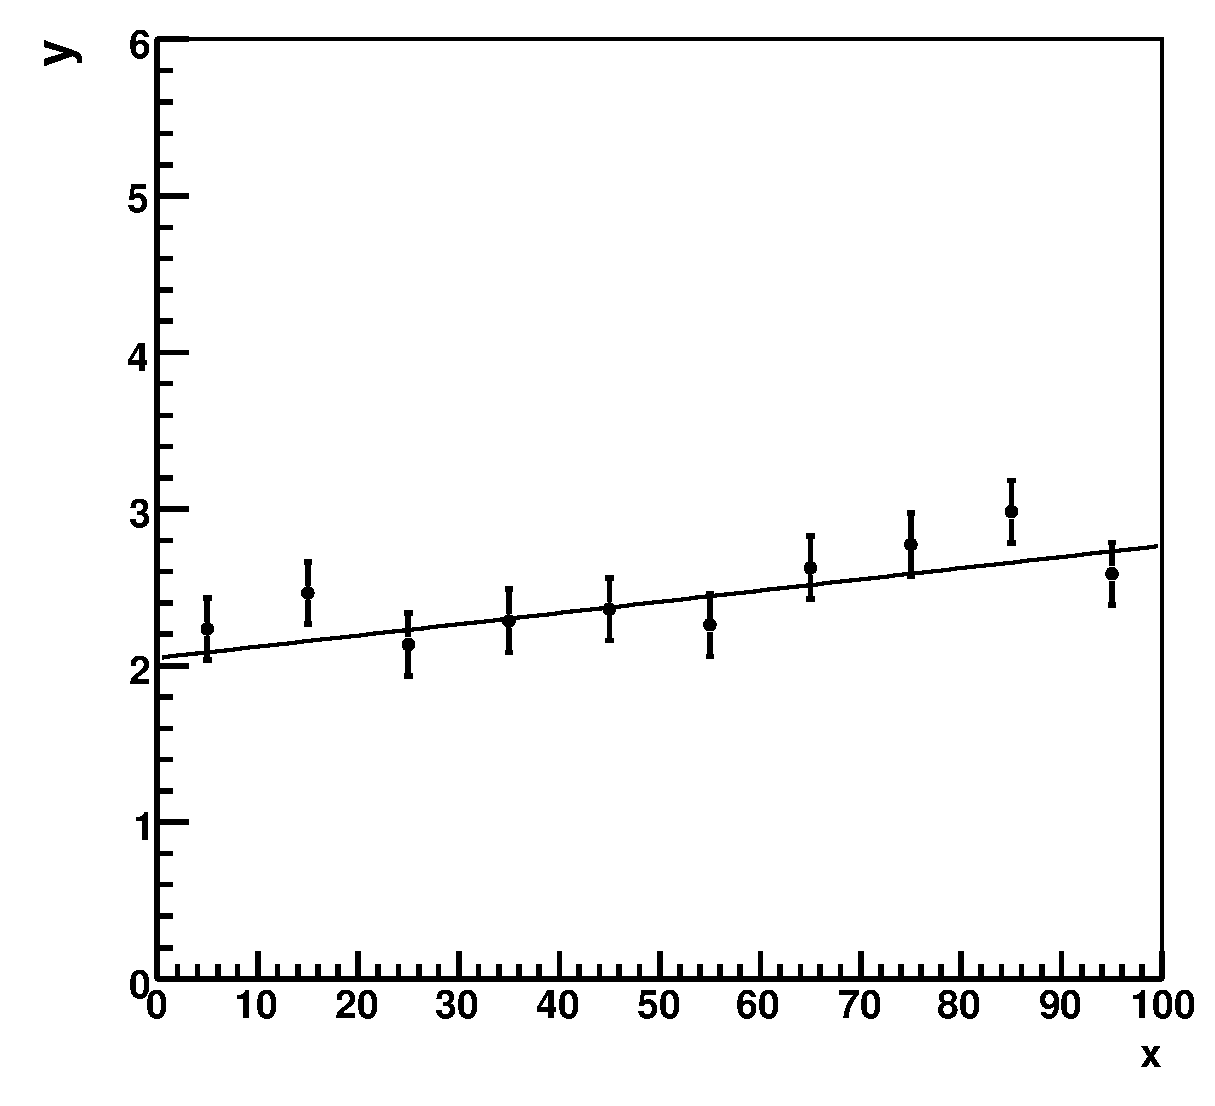
\includegraphics[height=4.0cm]{example01_data.eps}\end{minipage} & 
\begin{minipage}[t]{0.3\textwidth}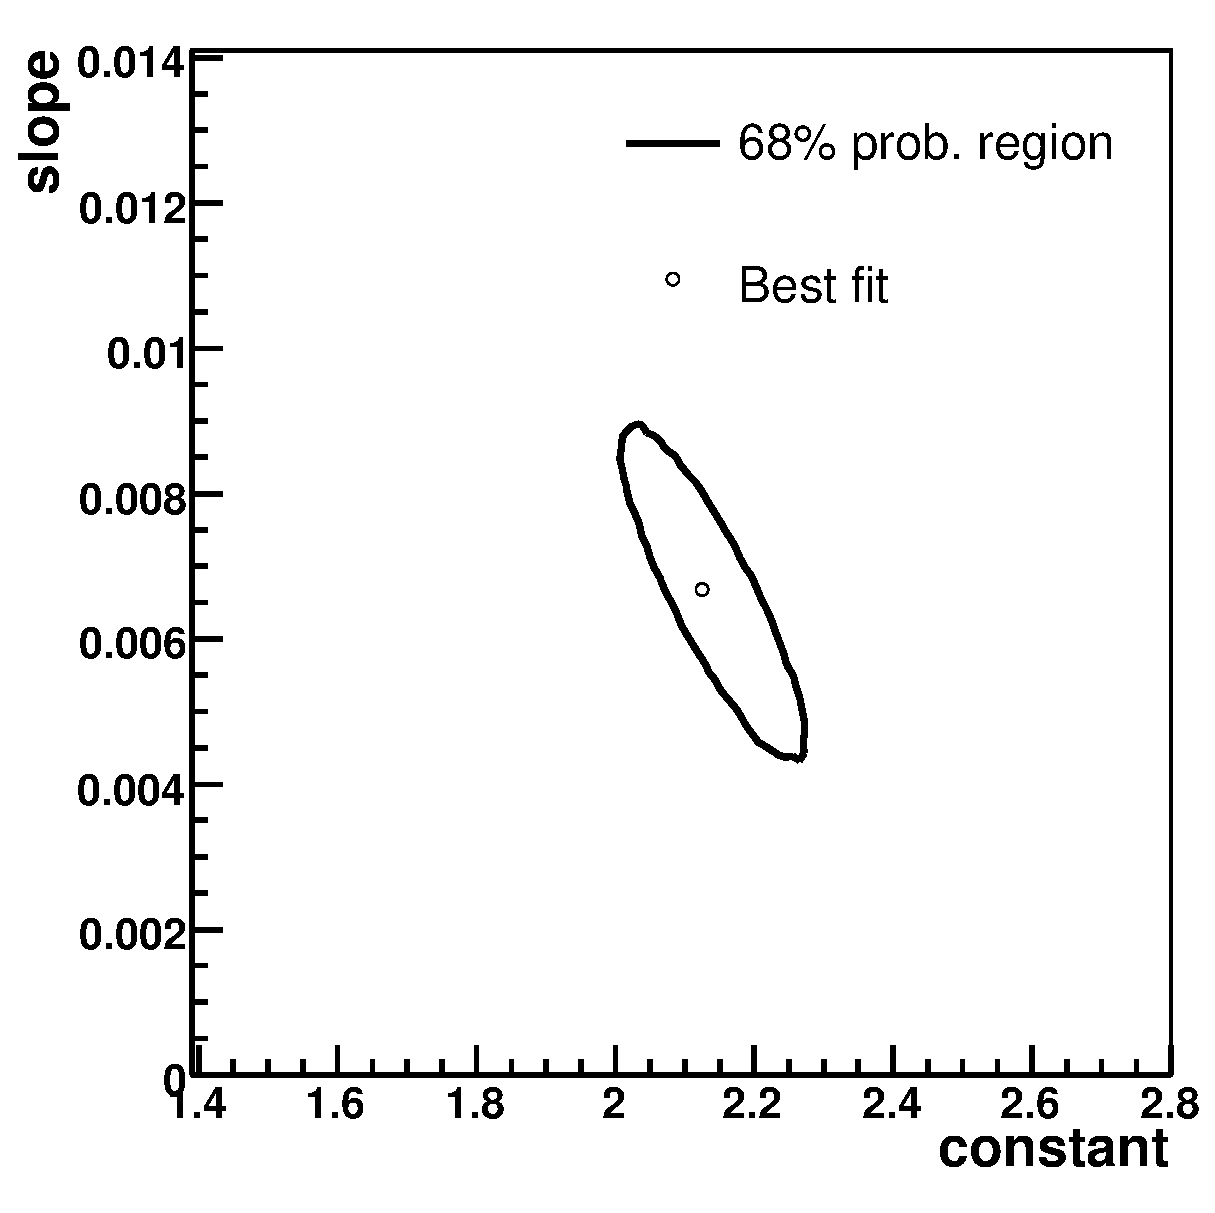
\includegraphics[height=4.0cm]{example01_correlation.eps}\end{minipage}  &
\begin{minipage}[t]{0.3\textwidth}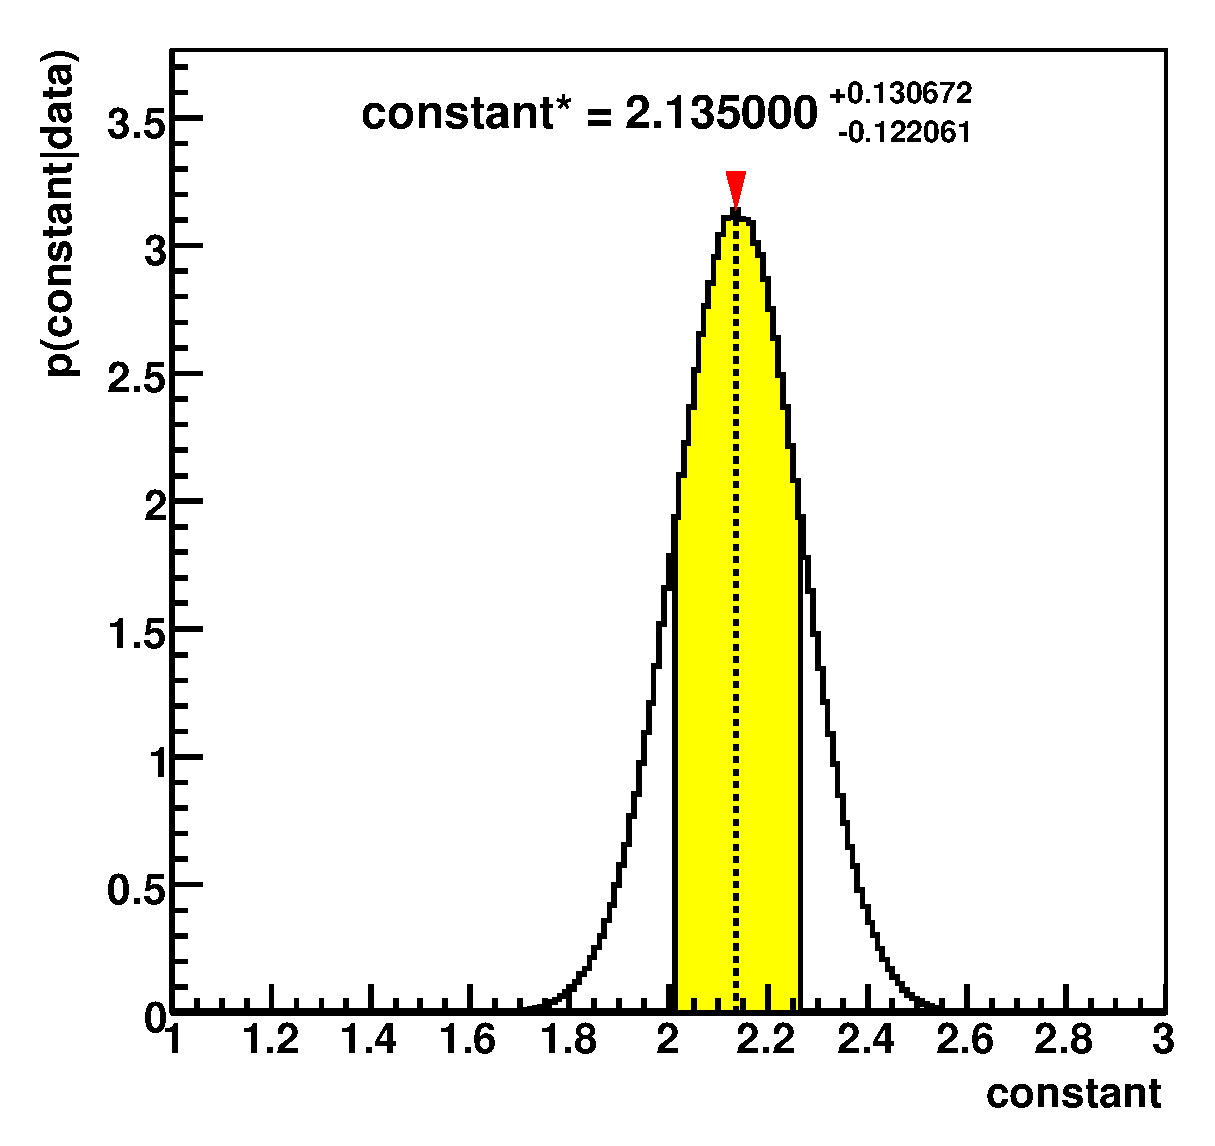
\includegraphics[height=4.0cm]{example01_constant.eps}\end{minipage} 
\end{tabular}
\caption{Left: Data set used in the example01 and best-fit straight line. Middle: Contour containing 68\% probability. Right: Marginalized probability density for the parameter constant. 
\label{fig:example01}}
\end{figure}

% --------------------------------------------------------

\subsection{Example 02: Polynomial fitting} 

As an extension of example~01 three different models are compared to
describe the data set. The difference between the model is the order
of the polynomial describing the correlation between the points:
constant, linear, quadratic. All three models are fitted to the data
and the a posteriori probability for the models is calculated. A
goodness-of-fit test is performed for the most probable model.

% --------------------------------------------------------

\subsection{Example 03: Spectral analysis} 
\label{section:example03} 

The data set is a binned spectrum with independent Poissonian
fluctuations in each bin. Two models for The underlying distribution
are compared: a background only distribution which is flat, and a
signal distribuion which has, in addition to a flat background, a
Gaussian peak at a defined position and with defined width. In the
former case, only the amount of background is a parameter while in the
latter case both, signal and background contribution, are parameters. 

% --------------------------------------------------------

\subsection{Example 04: Efficiency calculation} 

Given two numbers, $n$ and $k$, an efficiency is calculated as the
ratiom, $k/n$, of the two numbers. The one model implemented assumes
Poissonian fluctuations on $n$ and a Binomial distribution on $k$
given $n$. 

% --------------------------------------------------------
% bibliography 
% --------------------------------------------------------

\addcontentsline{toc}{section}{Bibliography}

\begin{thebibliography}{99}
%
\bibitem{Yao:2006px}
  W.~M.~Yao {\it et al.}  [Particle Data Group],
  ``Review of particle physics,''
  J.\ Phys.\ G {\bf 33} (2006) 1.
%
\bibitem{Schonert:2005zn}
  S.~Sch{\"o}nert {\it et al.}  [GERDA Collaboration],
  ``The GERmanium Detector Array (GERDA) for the search of neutrinoless beta
  beta decays of Ge-76 at LNGS,''
  Nucl.\ Phys.\ Proc.\ Suppl.\  {\bf 145} (2005) 242.
%
\bibitem{Caldwell:2006yj}
  A.~Caldwell and K.~Kr{\"o}ninger,
  ``Signal discovery in sparse spectra: A Bayesian analysis,''
  Phys.\ Rev.\  D {\bf 74}, 092003 (2006)
  [arXiv:physics/0608249].
%
\bibitem{ROOTweb}
http://root.cern.ch/
%
\bibitem{CUBA}
  T.~Hahn, ``CUBA: A library for multidimensional numerical
  integration,'' Comput.\ Phys.\ Commun.\ {\bf 168} (2005) 78
  [arXiv:hep-ph/0404043].
%
\bibitem{CUBAweb}
  http://www.feynarts.de/cuba/
%
\end{thebibliography}

\end{document} 


